




\chapter{Menu Edit}
\minitoc  

\section{Edit color and lighting options}

\noindent
The color and lighting options windows (Fig. \ref{color_options} p.\pageref{color_options}) makes it possible to edit the default solid color of newly opened surfaces, the background color of the upper part of the 3D window, and the background color of the lower part of the 3D window. The ambient, diffuse specular and specular power light settings can be set here as well. Four default presets combinations of ambient, diffuse specular lighting and power are available. Default color and light options can be reinitialized by pressing on the "Reinitialize" button. See Fig. \ref{lighting} p.\pageref{lighting} for an example of the impact of ambient, diffuse and specular light settings on rendering.

\begin{figure}
  \centering
  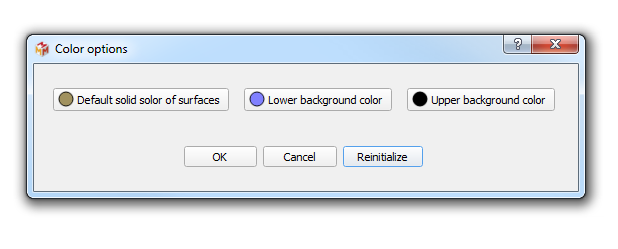
\includegraphics[scale=0.55]{images/08/color_options.png} 
	\caption{Color and lighting options window.}
\label{color_options}
 
\end{figure}

\begin{figure}
  \centering
  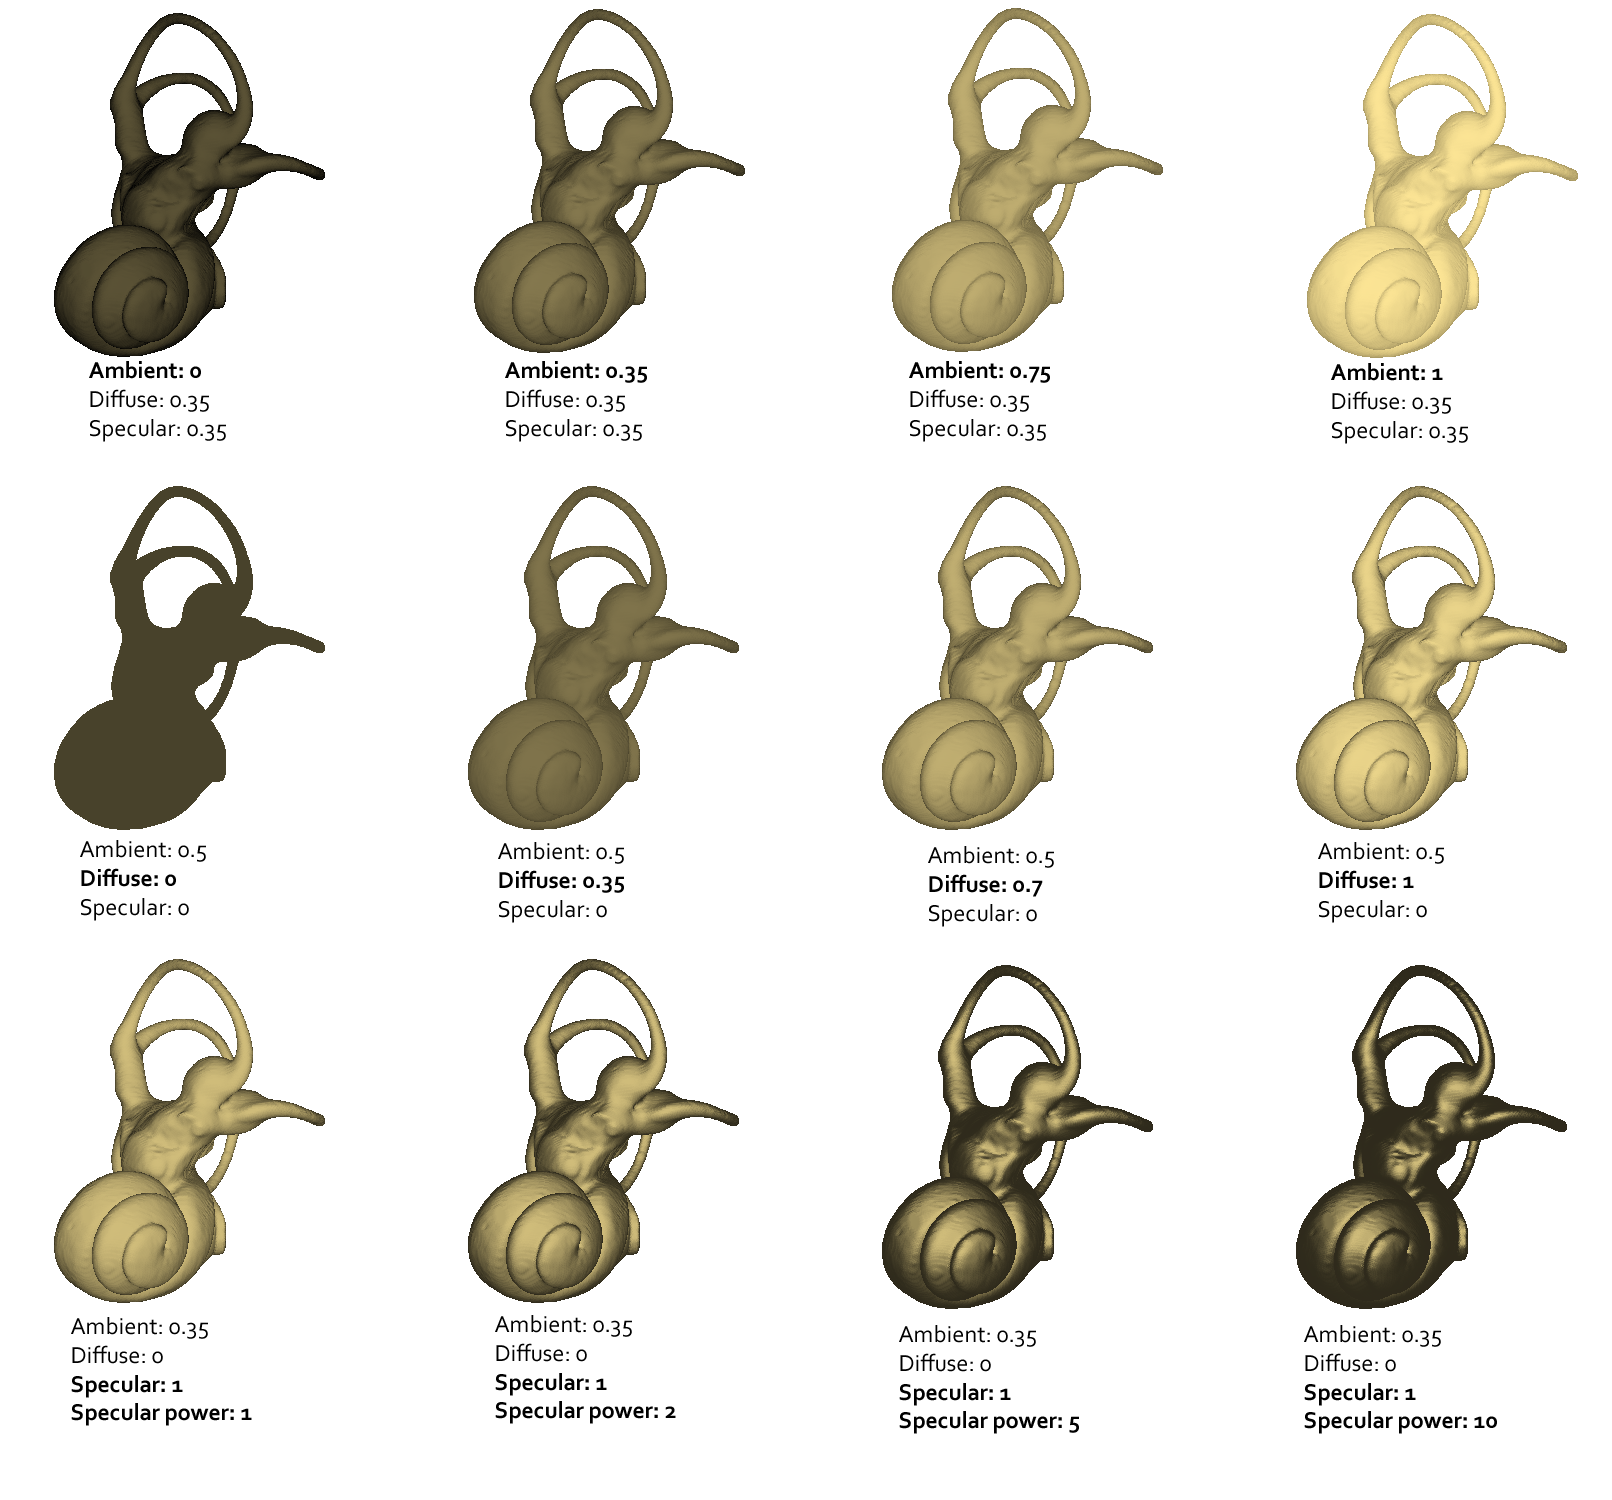
\includegraphics[scale=0.3]{images/08/lighting.png} 
	\caption{Different lighting parameters and resulting rendering of the 3D model of a left inner ear of \textit{Galago moholi}. \textbf{Top line:} modification of ambient lighting. \textbf{Middle line:} modification of diffuse lighting. \textbf{Bottom line:} modification of specular lighting.}
\label{lighting}
 
\end{figure}


\section{Edit size unit, grid spacing and scale}
\begin{figure}
  \centering
  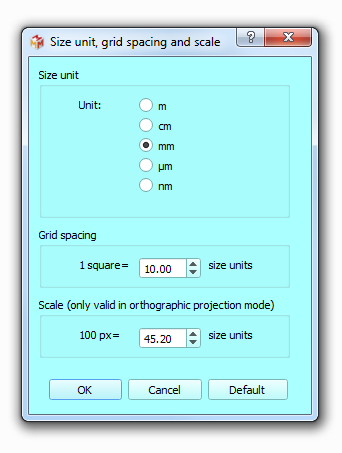
\includegraphics[scale=0.55]{images/08/size_unit_grid_spacing.png} 
	\caption{Size unit, grid spacing and scale window.}
\label{size_unit_grid_spacing}
 
\end{figure}

\noindent The "Size unit, grid spacing and scale" window (Fig. \ref{size_unit_grid_spacing} p.\pageref{size_unit_grid_spacing}) contains the following sections:\\\\
\subsection{Size unit}
\noindent MorphoDig's default size unit is "mm". 
However you can change the currently used size unit of your 3D surfaces. Indeed, different 3D surfaces may contain 3D x,y,z coordinates coded in different size units. Regarding 3D surfaces of biological models, one commonly used size-unit is  "mm". But 3D surfaces containing 3D x,y,z coordinates expressed in "\si{\micro}m" are also quite common. Be careful: MorphoDig will not be able to render at the correct scale two 3D surfaces using different 3D coordinates size units: if you have a first 3D surfaces expressed in "mm", and a second 3D surface expressed in "\si{\micro}m", the second surface will be rendered around 1000 times larger than the first one, and there is currently no straightforward way to detect which size unit is used for a given 3D surface. 


\subsection{Grid spacing}
\noindent You can change the rendering size of the grid. By default 1 grid is 10 mm. But depending on the size of your biological structure of interest, you may find it convenient to adjust grid display size to that of your 3D objects. 

\subsection{Scale (only valid in orthographic projection mode)}
\noindent As stated earlier, you can switch between orthographic and perspective projection mode by pressing the "
\includegraphics[scale=0.7]{images/06/camera/camera_ortho.png}" or "
\includegraphics[scale=0.7]{images/06/camera/camera_persp}" toggle button. In this section, you can adjust the display scale (=zoom) in order that 100 pixels on the screen translate into a desired number of size units in real world. This option is extremely useful to construct scale bars on scientific illustrations using software such as Gimp of Photoshop. For instance, if you set the display scale in order to have 100 pixels = 1 mm and then make a screenshot of your 3D objects in MorphoDig, if you want to place a scale bar of 5mm, you will simply have to create and draw a 500 pixel-wide rectangle over it. 




\noindent



\section{Landmark and flag rendering options}


The landmark and flag options window (see Fig. \ref{landmarks_flags_options} p.\pageref{landmarks_flags_options}) contains the following sections:
\begin{figure}
  \centering  
 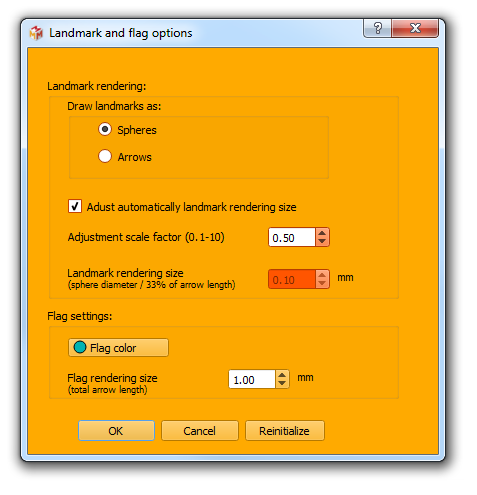
\includegraphics[scale=0.5]{images/08/landmark_flag_options.png}
 \captionof{figure}{Landmark and flag options window.}
\label{landmarks_flags_options}
\end{figure}

\begin{figure}
  \centering  
 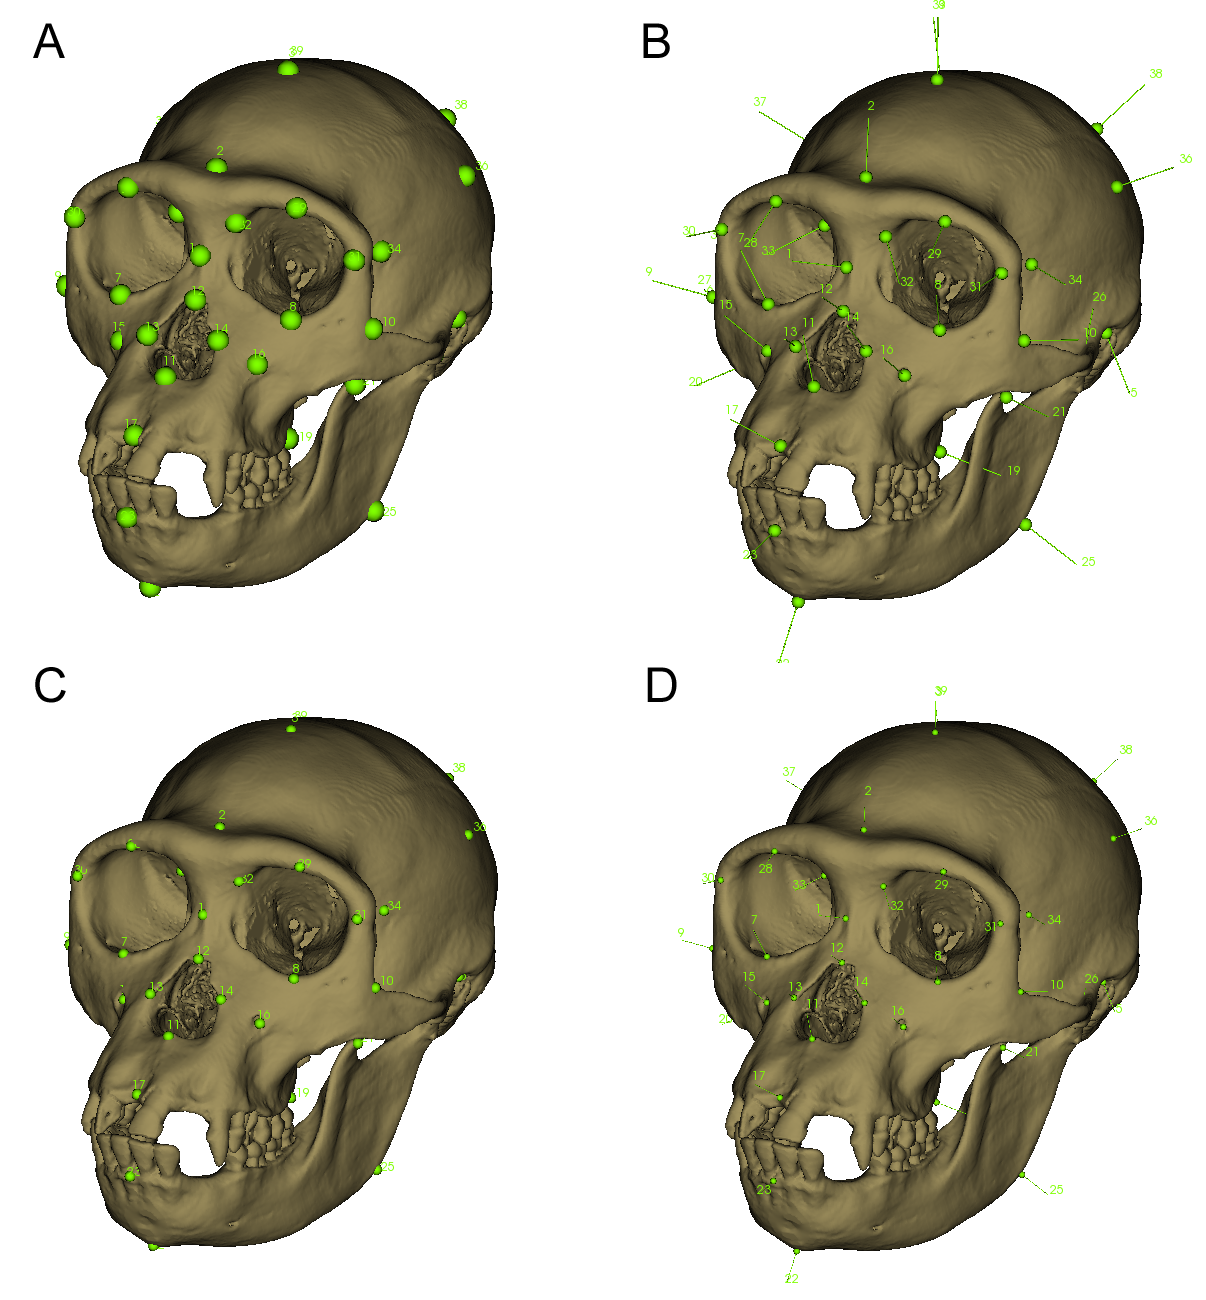
\includegraphics[scale=0.35]{images/08/landmark_rendering_option_example.png}
 \captionof{figure}{Example of the effect of different rendering options for the same set of landmarks (specimen: cranium and mandible of the type specimen of \textit{Pan paniscus}). A: Landmarks are drawn as spheres, rendering size is adjusted automatically, adjustment factor = 1. B: Landmarks are drawn as arrows, rendering size is adjusted automatically, adjustment factor = 1. C: Landmarks are drawn as spheres, rendering size is adjusted automatically, adjustment factor=0.5. D: Landmarks are drawn as arrows, rendering size is adjusted automatically, adjustment factor=0.5.}
\label{landmarks_flags_option_example}
\end{figure}
\subsection{Landmarks rendering}

``Normal", ``Target", ``Curve node" and ``Curve handle" landmarks can be drawn as spheres or as arrows (composed of a stick and a sphere). Landmark display size can be chosen to be adjusted automatically (default behaviour) and furthermore adjusted using an adjustment scale factor. Fig.  \ref{landmarks_flags_option_example} p.\pageref{landmarks_flags_option_example} shows the effect of the modification of this adjustment scale factor. Alternatively, you may decide to set manually landmark to a fixed rendering size.






\subsection{Flags settings}
Flag rendering size and flag color settings can be defined in this subsection. Once placed on a surface and selected, the color, the length and the label of the flag can be changed by pressing "
\includegraphics[scale=0.7]{images/06/objects/flag_edit.png}". This opens the "Edit first selected flag" window (Fig. \ref{flag_edit} p.\pageref{flag_edit}).




\section{Edit orientation labels}
\begin{figure}
  \centering  
 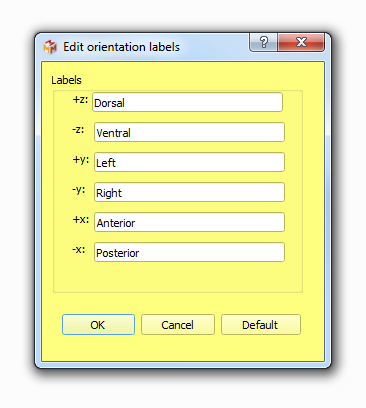
\includegraphics[scale=0.5]{images/08/orientation_labels.png}
 \captionof{figure}{Edit orientation labels window.}
\label{orientation_labels}
\end{figure}
The orientation labels of the orientation helper can be modified, or reinitialized to their default values via this menu (Fig. \ref{orientation_labels} p.\pageref{orientation_labels}).

As stated earlier, you can press 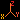
\includegraphics[scale=0.7]{images/06/display/orientation_helper.png} to show/hide the coordinate system orientation helper laying on the bottom left corner of the main 3D window.


\section{Edit camera options}
\begin{figure}
  \centering  
 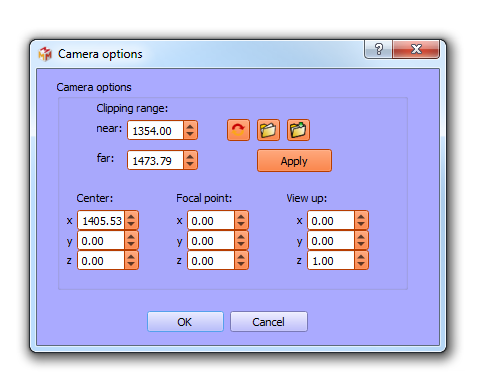
\includegraphics[scale=0.5]{images/08/camera_options.png}
 \captionof{figure}{Edit camera options window.}
\label{camera_options}
\end{figure}

The orientation and the position of the camera can be edited, saved, and imported in this section (Fig. \ref{camera_options} p.\pageref{camera_options}).
This can be useful when constructing a figure for a scientific publication, when you want to retrieve the exact position a screenshot was taken.